\documentclass{article}
\usepackage{arxiv}


\usepackage[utf8]{inputenc} 
\usepackage[T1]{fontenc}   
\usepackage{hyperref}       
\usepackage{url}          
\usepackage{booktabs}   
\usepackage{amsfonts}   
\usepackage{nicefrac}       
\usepackage{microtype}
\usepackage{graphicx}
\usepackage[style=apa]{biblatex}
\usepackage{doi}


\title{Detecting influential beliefs in large-scale surveys}
\author{ \href{https://orcid.org/0000-0003-4863-6051}{
\includegraphics[scale=0.06]{orcid.pdf}\hspace{1mm}Aleksandar Tomašević} \\
	Department of Sociology\\
	University of Novi Sad\\
	Novi Sad, Republic of Serbia\\
	\texttt{atomashevic@ff.uns.ac.rs}
}

\renewcommand{\shorttitle}{\textit{arXiv} Template}

\hypersetup{
pdftitle={Detecting influential beliefs in large-scale surveys},
pdfsubject={cs.SI,cs.CY,physics.soc-ph},
pdfauthor={Aleksandar Tomašević},
pdfkeywords={european social survey, belief system, network analysis, political networks},
}


\begin{document}

\maketitle

\section{Introduction}
\newpage
\section{Results}
\subsection{Unique variable analysis}

After two rounds of UVA redundancy detection
and the removal of 5 variables, we are left with the network with 10 nodes. Exploratory graph analysis confirmed the existence of a single community using Louvain algorithm and an extra unidimensionality check (which method?).

\begin{figure}[ht]
	\centering
	\label{fig:egafull}
	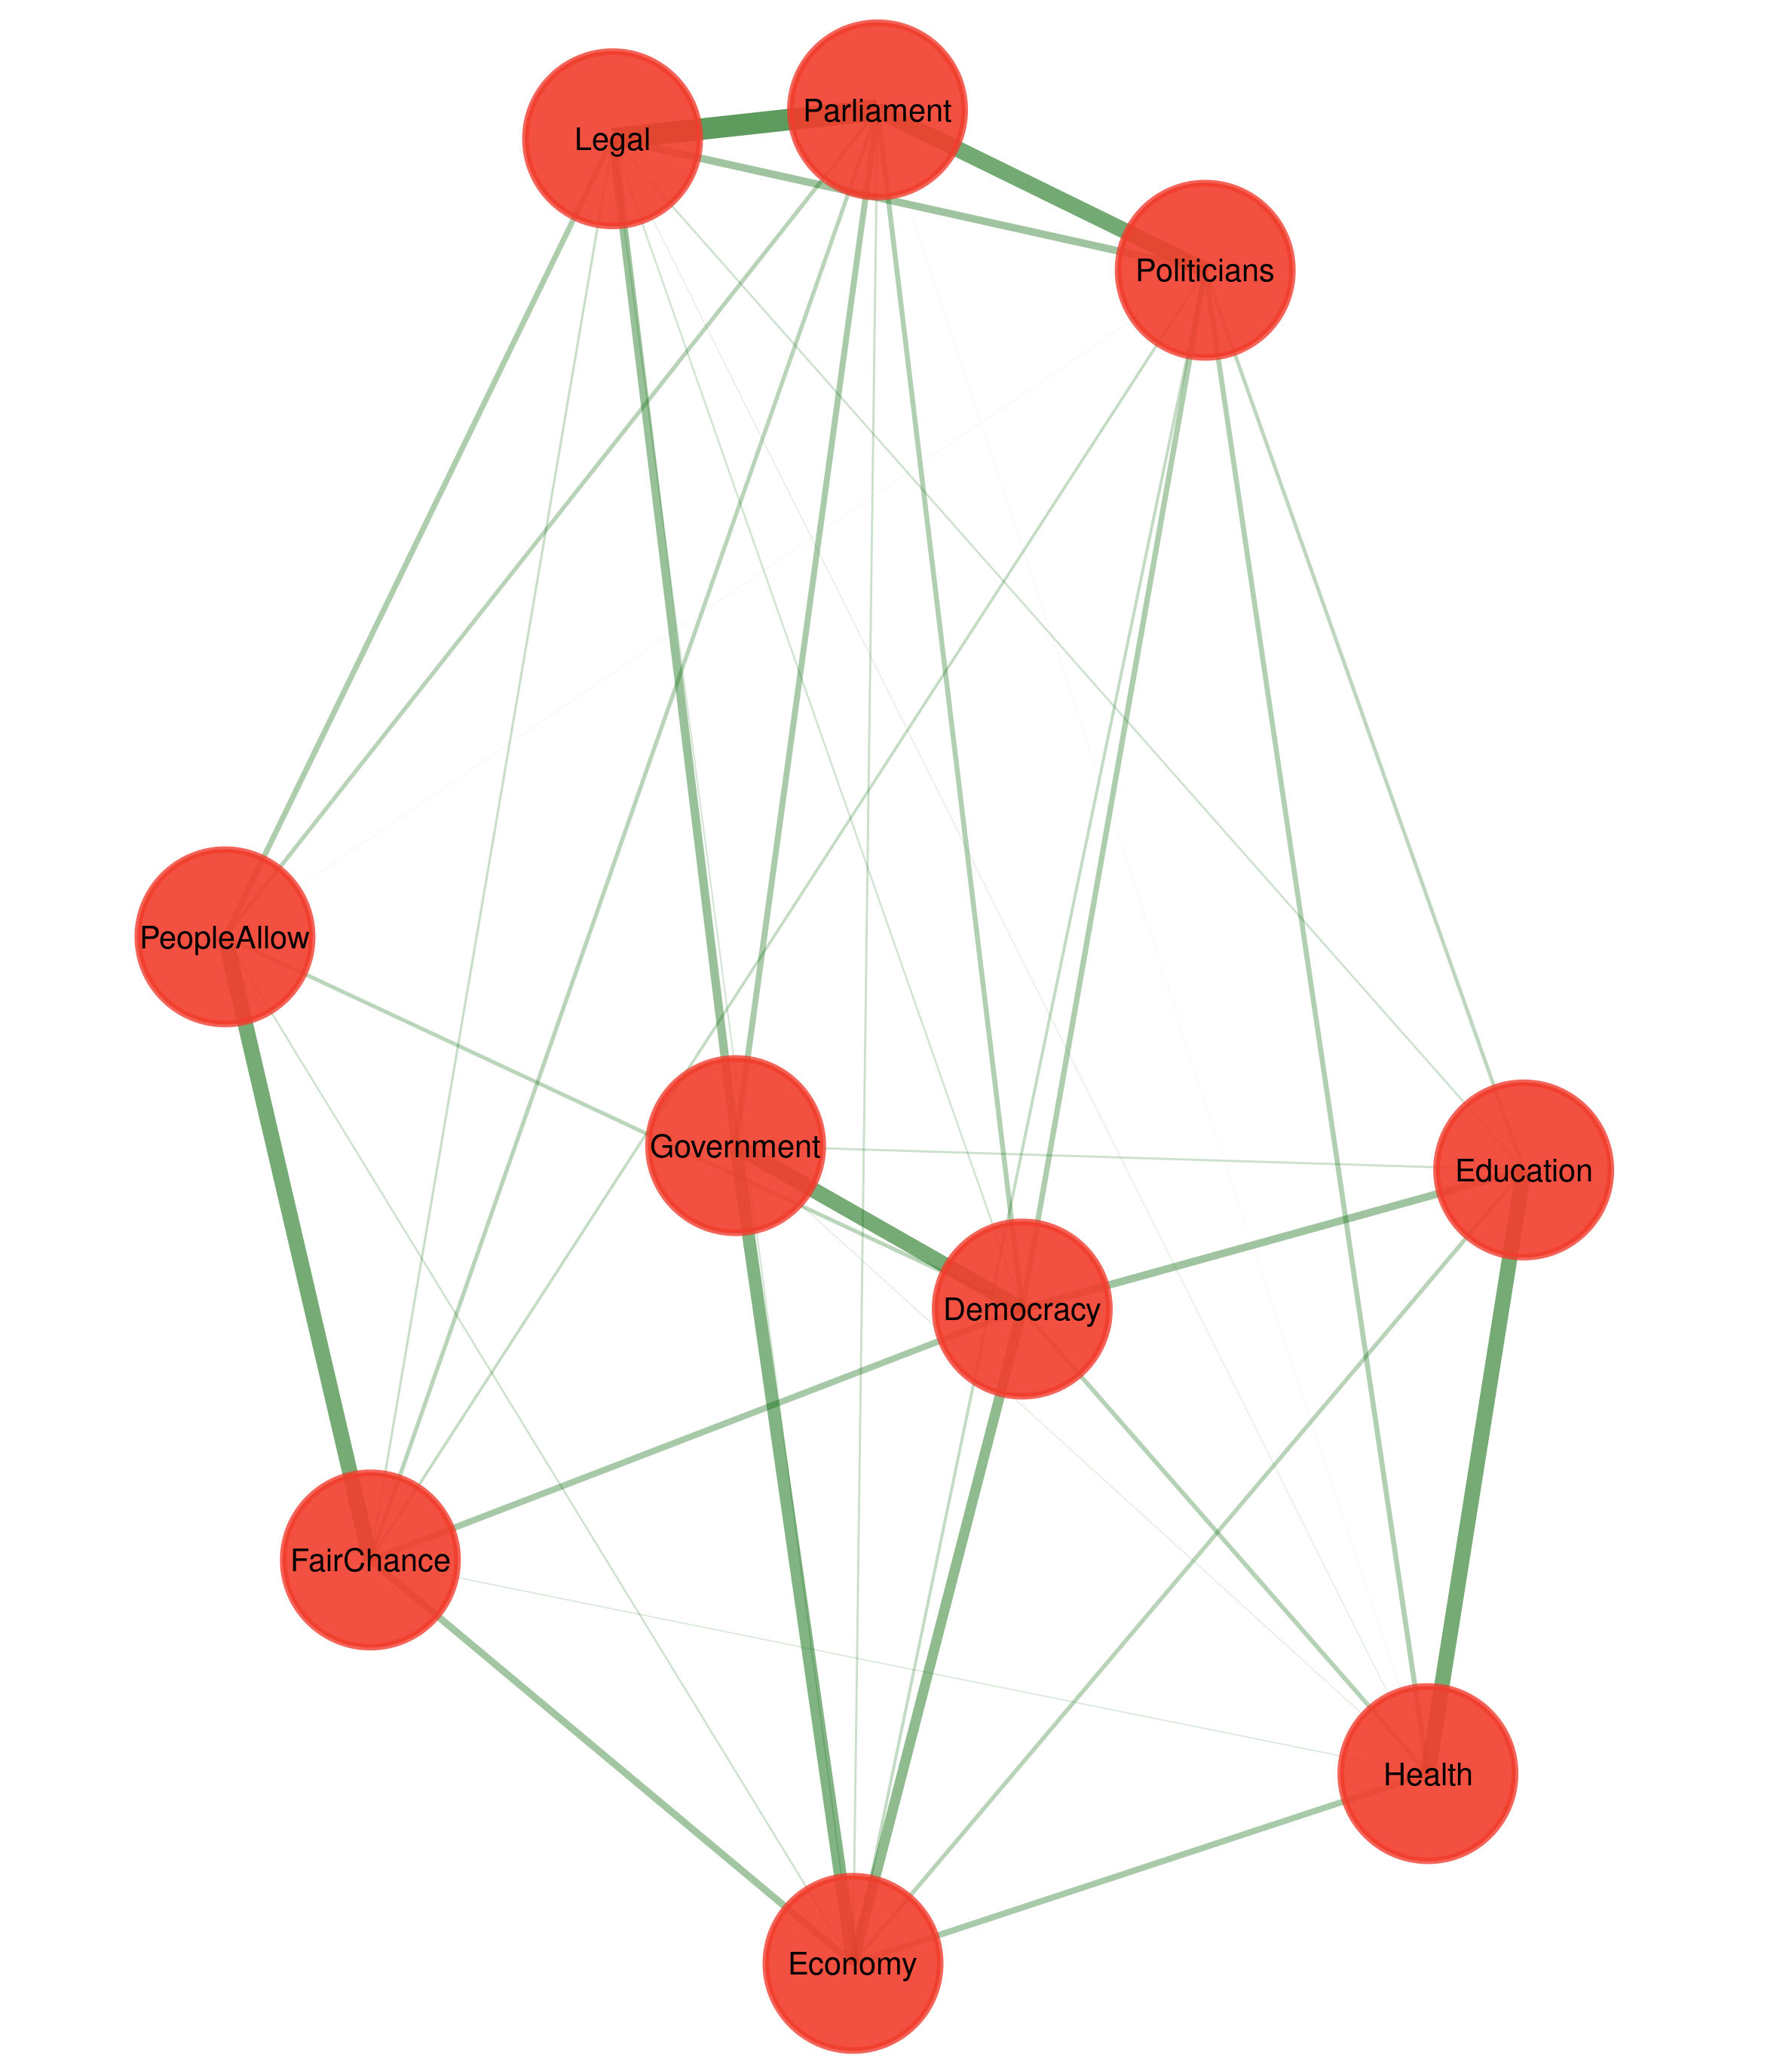
\includegraphics[width=0.5\textwidth]{figures/01-ega-full.png}
	\caption{Attitude network based on a complete dataset after redundancy analysis}
\end{figure}

\subsection{Intergrated Value of Influence}

Standardized values of IVI measure for the nodes of the network based on the complete dataset are shown on figure \ref{fig:ivifull}.

\begin{figure}[ht]
	\centering
	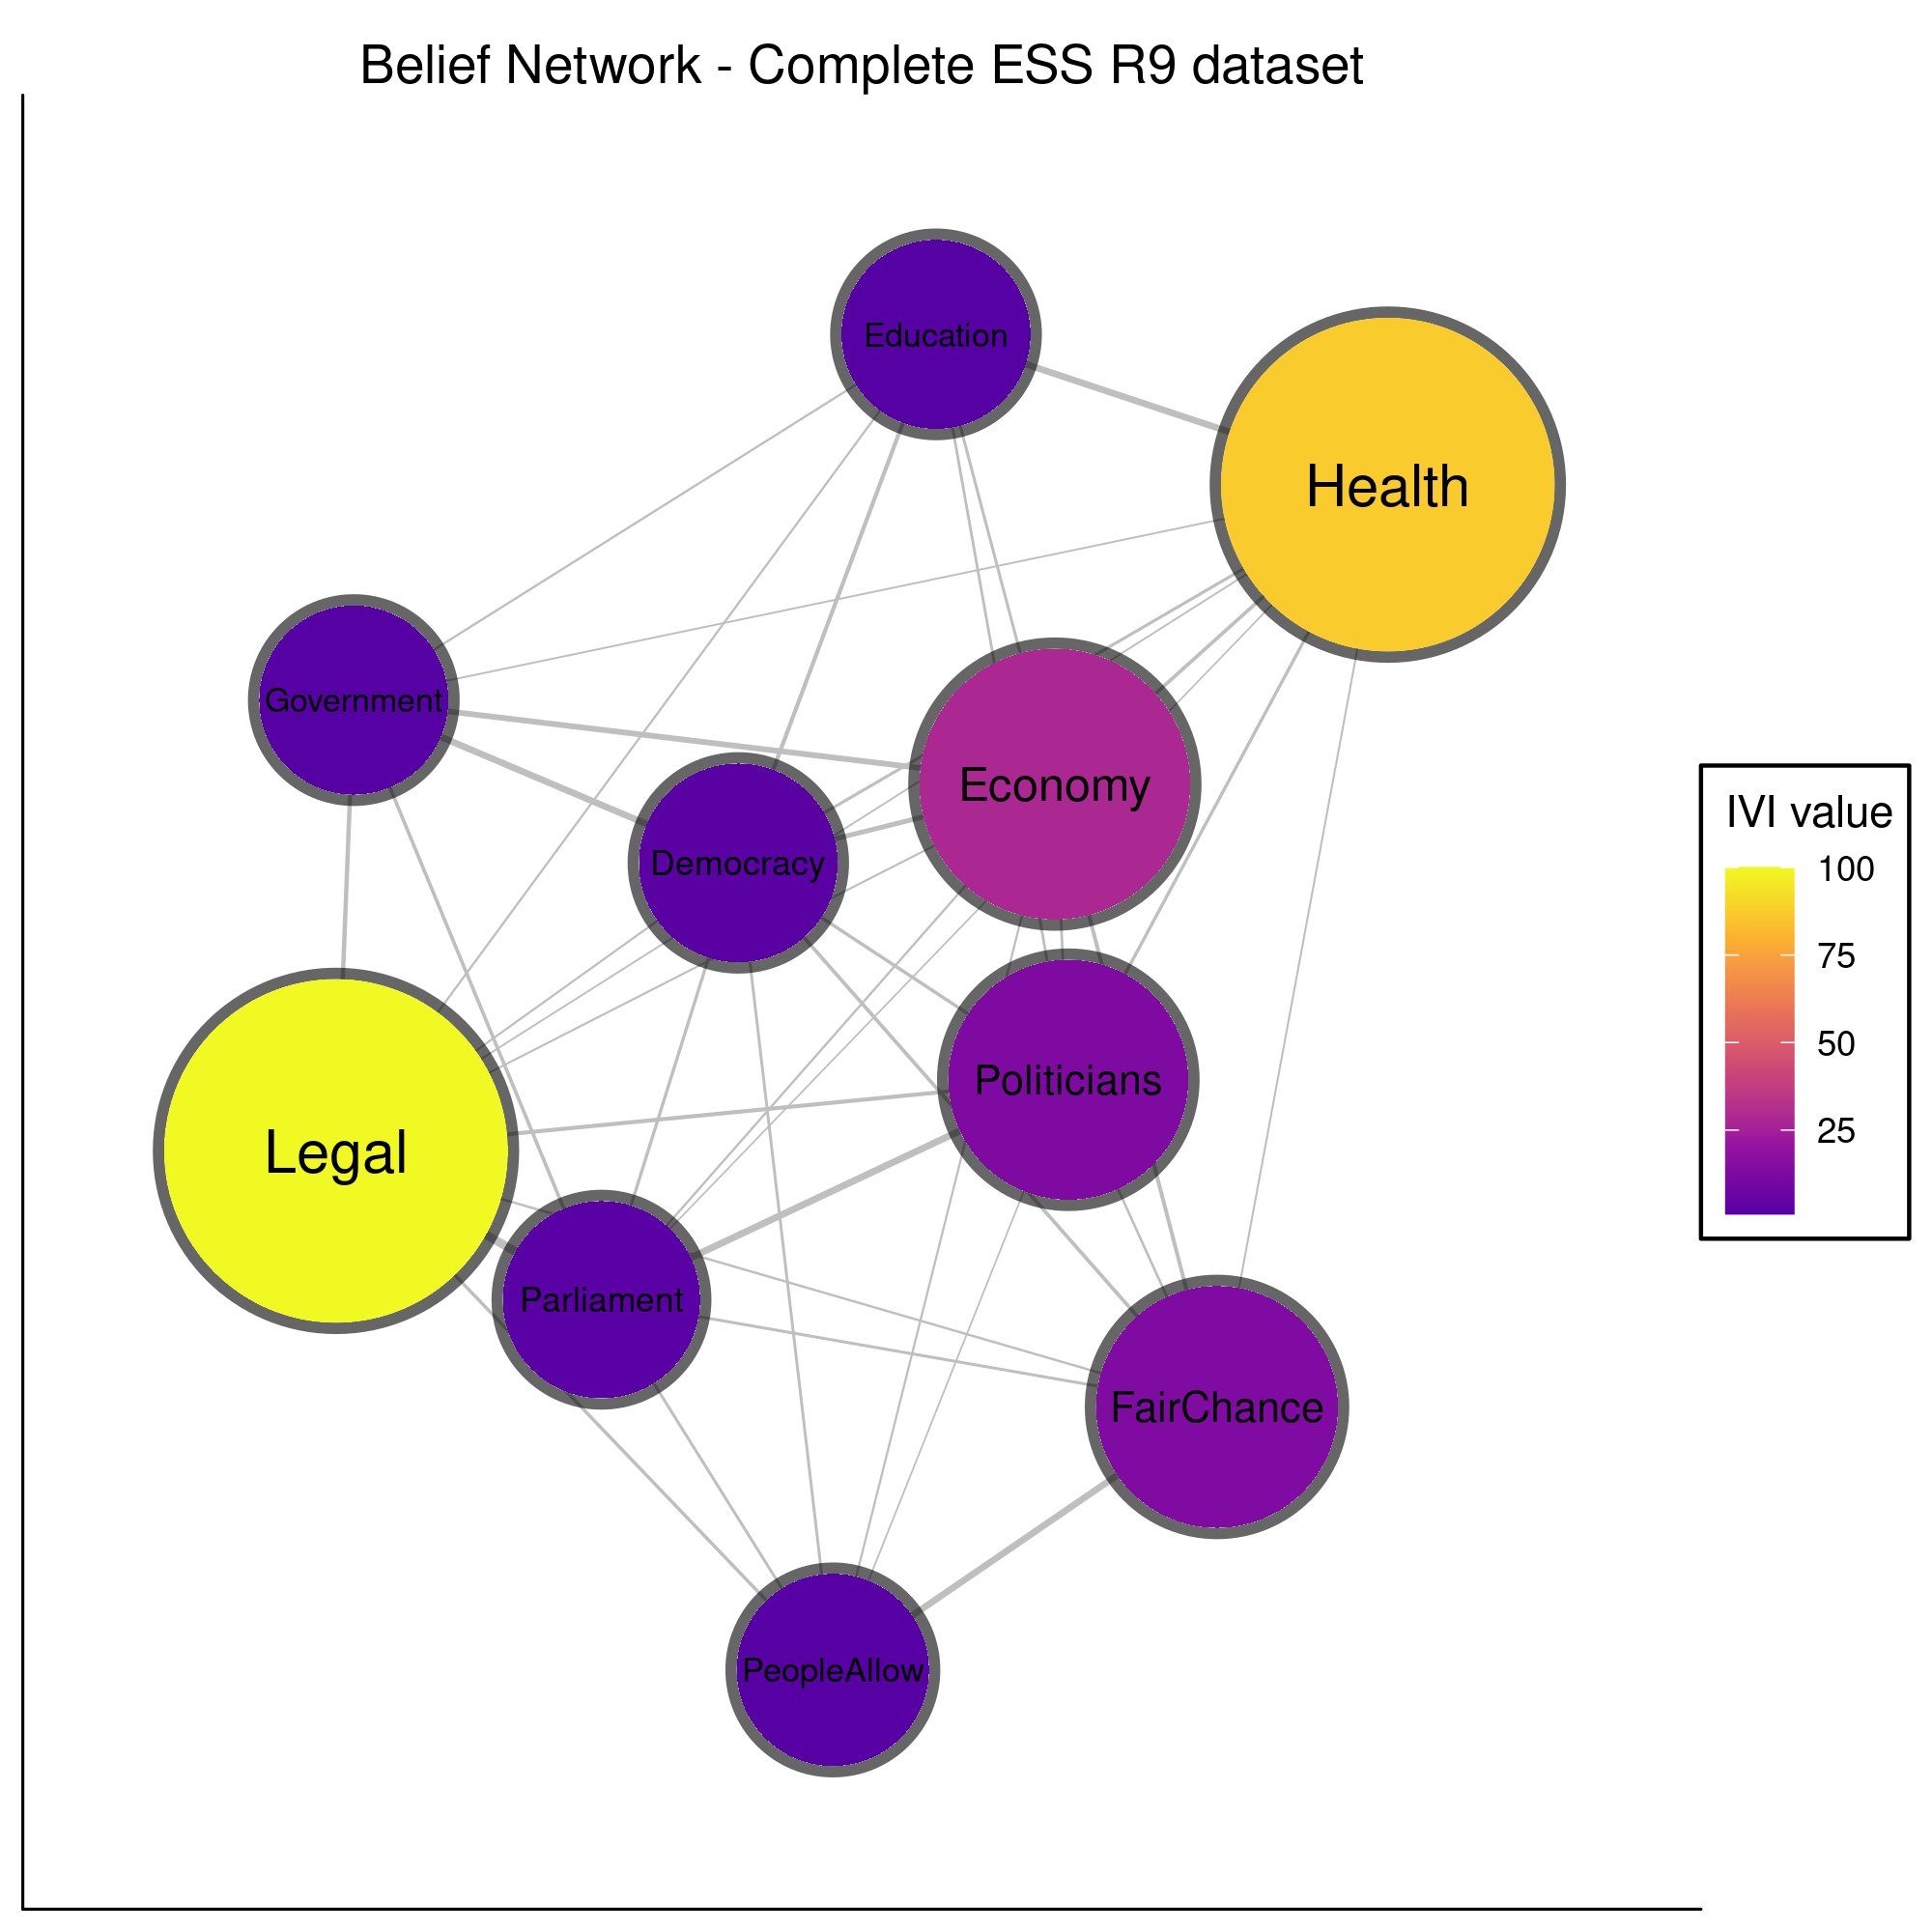
\includegraphics[width=0.5\textwidth]{figures/02-ivi-full.png}
	\label{fig:ivifull}
	\caption{Standardized IVI values for networks based on complete dataset}
\end{figure}



\end{document}
